\documentclass[a4paper, article, oneside, UKenglish]{memoir}
\usepackage{booktabs}
\usepackage{caption}
\usepackage{amsmath}
\usepackage{float}
\usepackage{graphicx}


%% Title page
\usepackage{projectfp}


%% Silence warning about obsolete package
\usepackage{silence}
\WarningFilter{remreset}{The remreset package}


%% Encoding
\usepackage[utf8]{inputenx} % Source code
\usepackage[T1]{fontenc}    % PDF


%% Fonts and typography
\usepackage{lmodern}           % Latin Modern Roman
\usepackage[scaled]{beramono}  % Bera Mono (Bitstream Vera Sans Mono)
\renewcommand{\sfdefault}{phv} % Helvetica
\usepackage[final]{microtype}  % Improved typography
\renewcommand{\abstractnamefont}{\sffamily\bfseries}                 % Abstract
\renewcommand*{\chaptitlefont}{\Large\bfseries\sffamily\raggedright} % Chapter
\setsecheadstyle{\large\bfseries\sffamily\raggedright}               % Section
\setsubsecheadstyle{\large\bfseries\sffamily\raggedright}            % Subsection
\setsubsubsecheadstyle{\normalsize\bfseries\sffamily\raggedright}    % Subsubsection
\setparaheadstyle{\normalsize\bfseries\sffamily\raggedright}         % Paragraph
\setsubparaheadstyle{\normalsize\bfseries\sffamily\raggedright}      % Subparagraph

%% Mathematics
\usepackage{amssymb}   % Extra symbols
\usepackage{amsthm}    % Theorem-like environments
\usepackage{thmtools}  % Theorem-like environments
\usepackage{mathtools} % Fonts and environments for mathematical formuale
\usepackage{mathrsfs}  % Script font with \mathscr{}


%% Miscellanous
\usepackage{graphicx}  % Tool for images
\graphicspath{{figures/}}
\usepackage{babel}     % Automatic translations
\usepackage{csquotes}  % Quotes
\usepackage{textcomp}  % Extra symbols
\usepackage{listings}  % Typesetting code
\lstset{basicstyle = \ttfamily, frame = tb}


%% Bibliography
\usepackage{mathscinet}
%\usepackage{biblatex}
%\usepackage[backend    = biber,
%            sortcites  = true,
%            giveninits = true,
%            doi        = false,
%            isbn       = false,
%            url        = false,
%            style      = alphabetic]{biblatex}
%\DeclareNameAlias{sortname}{family-given}
%\DeclareNameAlias{default}{family-given}
%\DeclareFieldFormat[article]{volume}{\bibstring{jourvol}\addnbspace#1}
%\DeclareFieldFormat[article]{number}{\bibstring{number}\addnbspace#1}
%\renewbibmacro*{volume+number+eid}
%{
%    \printfield{volume}
%    \setunit{\addcomma\space}
%    \printfield{number}
%    \setunit{\addcomma\space}
%    \printfield{eid}
%}
%\addbibresource{bibliography.bib}


%% Cross references
\usepackage{varioref}
\usepackage[pdfusetitle]{hyperref}
\urlstyle{sf}
\usepackage[nameinlink, capitalize, noabbrev]{cleveref}
\crefname{chapter}{Section}{Sections}


%% Theorem-like environments
\declaretheorem[style = plain, numberwithin = chapter]{theorem}
\declaretheorem[style = plain,      sibling = theorem]{corollary}
\declaretheorem[style = plain,      sibling = theorem]{lemma}
\declaretheorem[style = plain,      sibling = theorem]{proposition}
\declaretheorem[style = definition, sibling = theorem]{definition}
\declaretheorem[style = definition, sibling = theorem]{example}
\declaretheorem[style = remark,    numbered = no]{remark}


%% Delimiters
\DeclarePairedDelimiter{\p}{\lparen}{\rparen}   % Parenthesis
\DeclarePairedDelimiter{\set}{\lbrace}{\rbrace} % Set
\DeclarePairedDelimiter{\abs}{\lvert}{\rvert}   % Absolute value
\DeclarePairedDelimiter{\norm}{\lVert}{\rVert}  % Norm


%% Operators
\newcommand{\diff}{\mathop{}\!\mathrm{d}}
\DeclareMathOperator{\im}{im}
\DeclareMathOperator{\rank}{rank}
\DeclareMathOperator{\E}{E}
\DeclareMathOperator{\Var}{Var}
\DeclareMathOperator{\Cov}{Cov}


%% New commands for sets
\newcommand{\N}{\mathbb{N}}   % Natural numbers
\newcommand{\Z}{\mathbb{Z}}   % Integers
\newcommand{\Q}{\mathbb{Q}}   % Rational numbers
\newcommand{\R}{\mathbb{R}}   % Real numbers
\newcommand{\C}{\mathbb{C}}   % Complex numbers
\newcommand{\A}{\mathbb{A}}   % Affine space
\renewcommand{\P}{\mathbb{P}} % Projective space


%% New commands for vectors
\renewcommand{\a}{\mathbf{a}}
\renewcommand{\b}{\mathbf{b}}
\renewcommand{\c}{\mathbf{c}}
\renewcommand{\v}{\mathbf{v}}
\newcommand{\w}{\mathbf{w}}
\newcommand{\x}{\mathbf{x}}
\newcommand{\y}{\mathbf{y}}
\newcommand{\z}{\mathbf{z}}
\newcommand{\0}{\mathbf{0}}
\newcommand{\1}{\mathbf{1}}


%% Miscellanous
\renewcommand{\qedsymbol}{\(\blacksquare\)}


\title{Geostationary CubeSat Orbital Manoeuvre Feasibility Study (Preliminary Release)}
\author{Thomas Parry}
\revision{0}

\begin{document}


\projectfrontpage


\begin{abstract}
    \noindent
    The feasibility of raising a 6U CubeSat orbit from LEO (Low Earth Orbit) and GTO (Geosynchronous Transfer Orbit) to GEO (GEostationary Orbit) is investigated. The basic governing equations for the orbital manoeuvres are presented and manipulated to arrive at equations which can be used for initial thruster requirements.  
    
    Requirements for the thruster are calculated using cursory satellite constraints.  After a search of currently available thrusters the three best candidates are presented and compared to the derived requirements.  
    
    The initial conclusion is that orbital raising from LEO is not feasible, but with a GTO insertion orbit it is possible to meet the mission requirements.
    
    \textit{This is a preliminary release, the final release will include simulation results from NASA's GMAT software.}
\end{abstract}

\newpage

\chapter{Introduction}


This document presents an initial feasibility study of the orbital manoeuvres required to raise the Phase 4 Space satellite from an initial insertion orbit to an operational geostationary orbit.  Starting orbits in both LEO and GTO are analysed and the requirements on the thruster compared to what's currently available in the market.



\chapter{Governing Equations}

\section{Orbital Momentum, Period and Velocity}

The standard gravitational parameter, $ \mu $, is defined by in equation \ref{equ:mu_definition}. Where $ G $ is the gravitational constant and $ M $ is the mass of body the satellite is orbiting. As the analysis in this report is only concerned with earth orbits $ \mu $ is a constant.

\begin{equation}
\mu = GM = 3.986004418 \times 10^{14} ~~ (for ~ earth)
\label{equ:mu_definition}
\end{equation}

\begin{table}[h]
\centering
\begin{tabular}{@{}llll@{}}
\toprule
Orbit 		& Altitude (Apogee/Perigee)	& Radius (Apogee/Perigee) \\ \midrule
"Low" LEO   & 400 / 400~km				& 6,771 / 6,771~km   	\\
"High" LEO	& 800 / 800~km				& 7,171 / 7,171~km      \\
GTO      	& 36,000 /  200~km			& 42,371 / 6,571~km		\\
GEO      	& 35,786 / 35,786~km		& 42,371 / 42,371~km     \\ \bottomrule
\end{tabular}
\captionsetup{justification=centering}
\caption{Orbit altitudes and radii}
\label{tab:orbital_altitudes}
\end{table}

An orbit has a high point called apoapsis (apogee for earth orbits) and a low point called the periapsis (perigee for earth orbits).  The ratio between the apoapsis and periapsis is called the eccentricity which is defined in equation \ref{equ:eccentricity}.  For circular orbits the eccentricity, $e$, is equal to zero.

\begin{equation}
e = \frac{ r_a - r_p }{ r_a + r_p }
\label{equ:eccentricity}
\end{equation}

The semi-major axis is the average of the apogee and perigee as defined in equation \ref{equ:semimajor_axis}.

\begin{equation}
a = \frac{r_p + r_a}{2}
\label{equ:semimajor_axis}
\end{equation}

Using equation \ref{equ:eccentricity} and \ref{equ:semimajor_axis} the eccentricity and semi-major axis of each orbit is calculated and presented in table \ref{tab:orbital_eccentricities}.

\begin{table}[h]
\centering
\begin{tabular}{@{}lll@{}}
\toprule
Orbit 		& Eccentricity	& Semi-major Axis	\\ \midrule
"Low" LEO   & 0				& 6,771~km			\\
"High" LEO	& 0				& 7,171~km			\\
GTO      	& 0.731			& 24,471~km			\\
GEO      	& 0				& 42,371~km			\\ \bottomrule
\end{tabular}
\captionsetup{justification=centering}
\caption{Orbit eccentricities and semi-major axis}
\label{tab:orbital_eccentricities}
\end{table}

The angular momentum, $ \vec {L} $, of the orbiting satellite is defined in equation \ref{equ:angular_momentum} for a circular orbit with a position vector $ \vec{r} $ (with radius $r = r=\left\vert \vec{r} \right\vert)$), mass, $m$, and velocity, $\vec{v}$.

\begin{equation}
\vec{L} = \vec{r} \times m \vec{v}
\label{equ:angular_momentum}
\end{equation}

The specific angular momentum is normalised by the mass of the orbiting body (the satellite).

\begin{equation}
\vec{h} = \frac{\vec{L}}{m}
\label{equ:specific_angular_momentum}
\end{equation}

It is possible to arrive at a definition of the specific angular momentum defined in terms of the useful orbital parameters shown in equation \ref{equ:specific_angular_momentum_orbital}.  The specific angular momentum is constant throughout the orbit.

\begin{equation}
h = \sqrt{ \mu ~ r ~ (1 + e ~ cos( \theta )) }
\label{equ:specific_angular_momentum_orbital}
\end{equation}

\begin{table}[h]
\centering
\begin{tabular}{@{}ll@{}}
\toprule
Orbit 		& Angular Momentum			\\ \midrule
"Low" LEO   & $ 5.19512 \times 10^{10} ~~ m^2 \cdot s^{-1}$	\\
"High" LEO	& $ 5.34637 \times 10^{10} ~~ m^2 \cdot s^{-1}$	\\
GTO      	& $ 6.74030 \times 10^{10} ~~ m^2 \cdot s^{-1}$	\\
GEO      	& $ 1.29958 \times 10^{11} ~~ m^2 \cdot s^{-1}$	\\ \bottomrule
\end{tabular}
\captionsetup{justification=centering}
\caption{Orbit specific angular momentum}
\label{tab:orbital_momentum}
\end{table}



The orbital period is given by 

\begin{equation}
T = \frac{2 \pi}{\mu^2} {\left( \frac{h}{ \sqrt{1 - e^2} } \right)}^3
\label{equ:orbital_period}
\end{equation}


\begin{table}[h]
\centering
\begin{tabular}{@{}lllll@{}}
\toprule
Orbit 		Orbital Period 			\\ \midrule
"Low" LEO   & 92~min / 0.06~days    \\
"High" LEO	& 101~min / 0.07~days   \\
GTO      	& 635~min / 0.44~days   \\
GEO      	& 14,400~min / 1~day	\\ \bottomrule
\end{tabular}
\captionsetup{justification=centering}
\caption{Orbit period}
\label{tab:orbital_periods}
\end{table}

\begin{equation}
v \approx \sqrt{ \frac{ \mu }{a} }
\label{equ:velocity_sma}
\end{equation}


where $ v $ is the orbital velocity, $ \mu = G M $ is the standard gravitational parameter ($G$ is the gravitional constant, $M$ is the mass of the earth) which equals $ \approx 3.986 \times 10^{14} $ for the earth and $ a $ is the length of the semimajor axis in meters.

\section{Inclination Change}

Given an initial velocity, $ V_i $, final velocity, $ V_f $, and angle change given by $ \theta $ is defined in \cite{orbitalmechanics_website} as:

\begin{equation}
\Delta v = \sqrt{ V_i^2 + V_f^2 - 2 V_i V_f ~ cos( \theta ) }
\label{equ:deltav_inclination_change}
\end{equation}


When dimensioning the propulsion system the common orbits parameters must be considered due to the likely use of a free or discounted launch.  Figure \ref{fig:inclination_histogram} shows a histogram of the inclinations pulled from \cite{ucsusa_database}.

\begin{figure}[h]
    \centering
    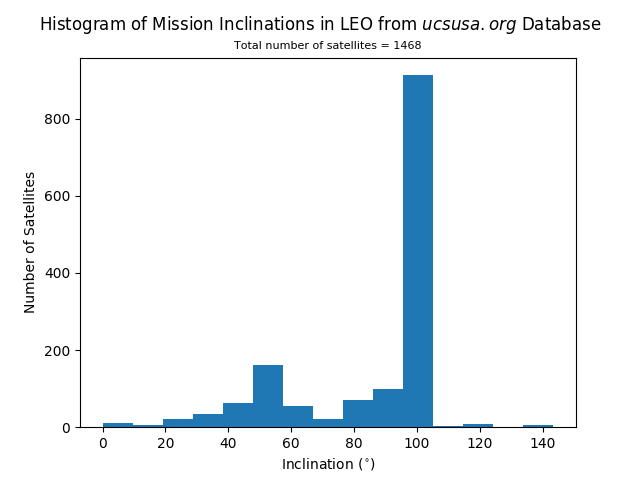
\includegraphics[width=\textwidth]{inclination_histogram}
    \caption{Distribution of orbit inclincations}
    \label{fig:inclination_histogram}
\end{figure}

There is a clear majority of satellites at an inclination of $ \approx 97^{\circ} $ which is a polar orbit used for earth observation applications.  This is a very poor inclination for the Phase 4 satellites as it requires a maximal inclination change. The second largest number of satellites is at an inclination of $ 51.6^{\circ} $, the same as the International Space Station because of the location of the primary US and Russian launch sites.

\section{Delta-V Requirements}

The total delta-V ($\Delta v$) required for the orbital manoeuvre is a key value to determine the requirements of the propulsion system.  

Newton's second law is rearranged as shown in equation \ref{equ:newtons_second} where $ F $ is the force of the thruster, $ m $ is the mass of the spacecraft and $ a $ is acceleration from the thruster burn (not to be confused with the semi-major axis with the same symbol).

\begin{equation}
\begin{split}
F = m \cdot a \\ 
a = \frac{F}{m}
\label{equ:newtons_second}
\end{split}
\end{equation}

The total $ \Delta v $ achieved over the period of the thruster burn, $T_{BURN}$, is the integral of the acceleration.  Using equation \ref{equ:newtons_second} the total $ \Delta v $ is found in equation \ref{equ:delta_v_integral}.

\begin{equation}
\Delta v = \int^{T_{BURN}} a \cdot dt = \int^{T_{BURN}} \frac{F}{m} \cdot dt = \frac{1}{m} \int^{T_{BURN}} F \cdot dt
\label{equ:delta_v_integral}
\end{equation}

For a thruster with a constant force the integral in equation \ref{equ:delta_v_integral} can be reduced to equation \ref{equ:delta_v_seconds}.

\begin{equation}
\Delta v =  \frac{1}{m} \cdot F \cdot T_{BURN}
\label{equ:delta_v_seconds}
\end{equation}

Finally, equation \ref{equ:thruster_force} will be used as the thruster selection criteria. 

\begin{equation}
F = \frac{\Delta v \cdot m}{T_{BURN}}
\label{equ:thruster_force}
\end{equation}



\chapter{Atmospheric Drag}

A rough expression for the atmospheric density is given in equation \ref{equ:air_density}.  Where the "Low LEO" case has an air density of $ 2.22 \times 10^{-12} ~ kg / m^3 $.

\begin{equation}
\rho = 1.02 \times 10^{7} \cdot {(0.001 \cdot a - 6,371)}^{-7.172}
\label{equ:air_density}
\end{equation}

The force exerted on the moving body in a viscous fluid (such as atmosphere) is shown in equation \ref{equ:air_force} where $A$ is the area of the satellite.

\begin{equation}
F = \rho A v^2
\label{equ:air_force}
\end{equation}

Equation \ref{equ:air_force} can be combined with equation \ref{equ:velocity_sma} to create the force on the satellite due to atmospheric drag at a given semi-major axis in equation \ref{equ:sma_drag_force}.  The force in "Low LEO" where area, $ A = 0.36 ~ m^2 $, from three 6U faces gives an atmospheric drag of $ \approx 47 ~ \mu N $.

\begin{equation}
F = \frac{\mu}{a} \cdot 1.02 \times 10^{7} \cdot {(0.001 \cdot a - 6,371)}^{-7.172}
\label{equ:sma_drag_force}
\end{equation}

Given the thruster force is likely to be greater than $ 1 ~ mN $ the atmospheric drag can (to first order) be ignored is a fast ascent (< 1 year) is assumed.  As the atmospheric density drops exponentially with altitude the effect is even less pronounced once the satellite leaves low earth orbit.



\chapter{LEO to GEO}

\section{$\Delta v$ Requirements}

The $ \Delta v $ required from a circular orbit in LEO to GEO is plotted in figure \ref{fig:deltav_contour}.  The impact of the initial inclination can be seen where the $ \Delta v$ required from an inclination of $\approx 100^{\circ}$ is approximately double that required from an inclination of $0^{\circ}$.

\begin{figure}[H]
    \centering
    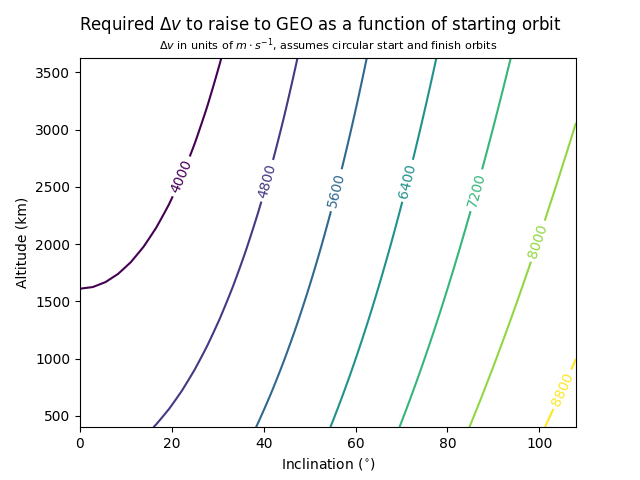
\includegraphics[width=\textwidth]{deltav_contour}
    \caption{$\Delta v$ required to move to GEO from LEO}
    \label{fig:deltav_contour}
\end{figure}

For more detail the $ \Delta v $ for varying initial altitudes for both inclinations of $0^{\circ}$ and $52^{\circ}$ are shown in figures \ref{fig:deltav_incl0} and \ref{fig:deltav_incl52} respectively.

\begin{figure}[H]
    \centering
    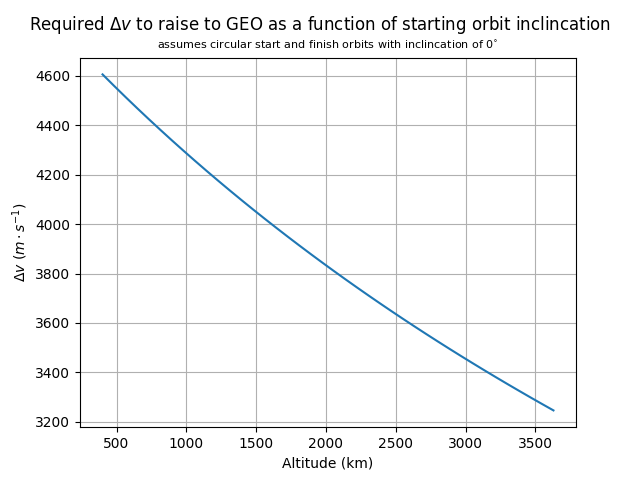
\includegraphics[width=\textwidth]{deltav_incl0}
    \caption{$\Delta v$ required to move to GEO from LEO from inclination of $0^{\circ}$}
    \label{fig:deltav_incl0}
\end{figure}


\begin{figure}[H]
    \centering
    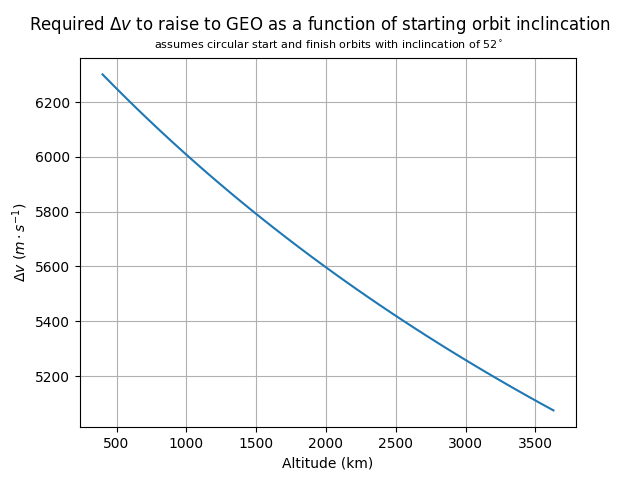
\includegraphics[width=\textwidth]{deltav_incl52}
    \caption{$\Delta v$ required to move to GEO from LEO from inclination of $52^{\circ}$}
    \label{fig:deltav_incl52}
\end{figure}







\section{Propulsion Requirements}

To derive the propulsion requirements the constraints of the mission must first be defined.  These parameters are shown in table \ref{tab:leo_to_geo_definition} and are meant to represent a typical 6U from a low cost launch opportunity.

\begin{table}[h]
\centering
\begin{tabular}{@{}lllll@{}}
\toprule
Parameter					& Value			\\ \midrule
CubeSat Size				& $6U$			\\
Mass  						& $10~kg$		\\
Insertion Orbit Altitude	& $400~km$		\\
Insertion Orbit Inclination	& $57^\circ$	\\
Maximum Manoeuvre Duration 	& $1~year$		\\ \bottomrule
\end{tabular}
\captionsetup{justification=centering}
\caption{LEO to GEO mission definition}
\label{tab:leo_to_geo_definition}
\end{table}

The following sections will use the information and calculations presented in the previous sections to arrive at the final thruster requirements.


\subsection{Altitude $\Delta V$}

Using equation \ref{equ:velocity_sma} the initial and final velocities are calculated in equations \ref{equ:leo_initial_v} and \ref{equ:leo_final_v}

\begin{equation}
v_i \approx \sqrt{ \frac{ \mu }{a} } = \sqrt{ \frac{ 3.986004418 \times 10^{14} }{6.771 \times 10^{6}} } = 7672~ms^{-1}
\label{equ:leo_initial_v}
\end{equation}

\begin{equation}
v_f \approx \sqrt{ \frac{ \mu }{a} } = \sqrt{ \frac{ 3.986004418 \times 10^{14} }{4.2371 \times 10^{7}} } = 3067~ms^{-1} 
\label{equ:leo_final_v}
\end{equation}


\subsection{Total $\Delta V$}

Using equation \ref{equ:deltav_inclination_change} the total $ \Delta v $ required is calculated in equation \ref{equ:leo_deltav}.

\begin{equation}
\begin{split}
\Delta V = \sqrt{ V_i^2 + V_f^2 - 2 V_i V_f ~ cos( \theta ) } \\ 
= \sqrt{ 7672^2 + 3067^2 - 2 \cdot 7672 \cdot 3067 \cdot cos( 57^{\circ} ) } \\
= 6,530~ms^{-1}
\end{split}
\label{equ:leo_deltav}
\end{equation}


\subsection{Total Impulse}

The total impulse is a measure of the total amount of momentum change and allows the selection of an appropriate thruster.  The total impulse is calculated in equation \ref{equ:leo_thruster_force}.

\begin{equation}
J = \Delta v \cdot m = 6,530 \cdot 10 = 65,300 ~ kg \cdot ms^{-1}
\label{equ:leo_total_impulse}
\end{equation}


\subsection{Required Thrust}

Finally we can calculate the required thrust to make the orbital manoeuvre in the required time frame using equation \ref{equ:leo_thruster_force}.

\begin{equation}
F = \frac{\Delta v \cdot m}{T_{BURN}} = \frac{6,530 \cdot 10}{1 \cdot 365 \cdot 24 \cdot 60 \cdot 60} = 2 ~ mN
\label{equ:leo_thruster_force}
\end{equation}


\subsection{Requirements Summary}

In summary the two requirements (excluding spacecraft constraints such as volume, mass, power etc.) which allow a suitable thruster to be selected are shown in table \ref{tab:leo_to_geo_thruster_requirements}.

\begin{table}[h]
\centering
\begin{tabular}{@{}lllll@{}}
\toprule
Parameter					& Value							\\ \midrule
Thrust						& $> 2~mN$						\\
Total Impulse				& $65,300~kg \cdot ms^{-1}$	\\ \bottomrule
\end{tabular}
\captionsetup{justification=centering}
\caption{LEO to GEO mission thrust requirements}
\label{tab:leo_to_geo_thruster_requirements}
\end{table}

The thrust is a simple value to pull from a thruster datasheet.  However the total impulse will require some calculation using equation \ref{equ:total_impulse_calc} or represented with words below:
\\
\\
\centerline{\scalebox{0.9}{
$Total ~ Impulse = Specific ~ Impulse \cdot Gravitional ~ Constant \cdot Propellant ~ Mass$
}}

\begin{equation}
J = I_{SP} \cdot g_0 \cdot m_p ~~~~~~[kg \cdot ms^{-1}~~or~~ s \cdot g_0 \cdot kg]
\label{equ:total_impulse_calc}
\end{equation}

Note that the gravitional constant is equal to $ 9.8~ms^{-2} $.



\chapter{GTO to GEO}

The GTO insertion orbit mission constraints are presented in table \ref{tab:gto_to_geo_definition}.  The inclination was selected from the worst case shown in SpaceX's Falcon 9 for a GTO insertion \cite{falcon9}.

\begin{table}[h]
\centering
\begin{tabular}{@{}lllll@{}}
\toprule
Parameter						& Value			\\ \midrule
CubeSat Size					& $6U$			\\
Mass  							& $10~kg$		\\
Insertion Orbit Semi-Major Axis	& $24,471~km$	\\
Insertion Orbit Inclination		& $28.5^\circ$	\\
Maximum Manoeuvre Duration 		& $1~year$		\\ \bottomrule
\end{tabular}
\captionsetup{justification=centering}
\caption{LEO to GEO mission definition}
\label{tab:gto_to_geo_definition}
\end{table}


\subsection{Altitude $\Delta V$}

Using equation \ref{equ:velocity_sma} the initial and final velocities are calculated in equations \ref{equ:gto_initial_v} and \ref{equ:gto_final_v}

\begin{equation}
v_i \approx \sqrt{ \frac{ \mu }{a} } = \sqrt{ \frac{ 3.986004418 \times 10^{14} }{2.4471 \times 10^{7}} } = 4036~ms^{-1}
\label{equ:gto_initial_v}
\end{equation}

\begin{equation}
v_f \approx \sqrt{ \frac{ \mu }{a} } = \sqrt{ \frac{ 3.986004418 \times 10^{14} }{4.2371 \times 10^{7}} } = 3067~ms^{-1} 
\label{equ:gto_final_v}
\end{equation}


\subsection{Total $\Delta V$}

Using equation \ref{equ:deltav_inclination_change} the total $ \Delta v $ is calculated in equation \ref{equ:gto_final_v}

\begin{equation}
\begin{split}
\Delta V = \sqrt{ V_i^2 + V_f^2 - 2 V_i V_f ~ cos( \theta ) } \\ 
= \sqrt{ 4036^2 + 3067^2 - 2 \cdot 4036 \cdot 3067 \cdot cos( 28.5^{\circ} ) } \\
= 1,985~ms^{-1}
\end{split}
\label{equ:gto_deltav}
\end{equation}


\subsection{Total Impulse}

The total impulse is calculated in equation \ref{equ:leo_thruster_force}.

\begin{equation}
J = \Delta v \cdot m = 1,985 \cdot 10 = 19,850 ~ kg \cdot ms^{-1}
\label{equ:gto_total_impulse}
\end{equation}


\subsection{Required Thrust}

The optimum low thrust manoeuvre from GTO to GEO is an active area of research and more investigation is required to provide firm answers.  However some order of magnitude estimates can be made, looking at current research the thruster is only active for approximately a sixth of the orbit\cite{gto_to_geo}.  Adding 20\% implementation loss to the $\Delta v$ calculated in equation \ref{equ:gto_deltav} the required thrust is calculated in equation \ref{equ:gto_thruster_force}.

\begin{equation}
F = \frac{1.2 \cdot \Delta v \cdot m}{6 \cdot T_{BURN}} = \frac{1.2 \cdot 1,985 \cdot 10}{6 \cdot 1 \cdot 365 \cdot 24 \cdot 60 \cdot 60} = 126 ~ \mu N
\label{equ:gto_thruster_force}
\end{equation}

\subsection{Requirements Summary}

In summary the two requirements (excluding spacecraft constraints such as volume, mass, power etc.) which allow a suitable thruster to be selected are shown in table \ref{tab:gto_to_geo_thruster_requirements}.

\begin{table}[h]
\centering
\begin{tabular}{@{}lllll@{}}
\toprule
Parameter					& Value							\\ \midrule
Thrust						& $126 ~ \mu N$					\\
Total Impulse				& $19,850~kg \cdot ms^{-1}$		\\ \bottomrule
\end{tabular}
\captionsetup{justification=centering}
\caption{LEO to GEO mission thrust requirements}
\label{tab:gto_to_geo_thruster_requirements}
\end{table}



\chapter{GEO to Graveyard}

At end of life the satellite is required to move to a graveyard orbit to avoid occupation of a valuable geostationery orbit location.  The exact requirements for the graveyard orbit depend on the solar radiation pressure coefficient of the satellite but for this initial feasibility study an altitude 300 km above geostationary orbit is used.

\begin{table}[h]
\centering
\begin{tabular}{@{}lllll@{}}
\toprule
Parameter						& Value			\\ \midrule
CubeSat Size					& $6U$			\\
Mass  							& $10~kg$		\\
Starting Orbit Semi-Major Axis	& $42,371~km$	\\
Final Orbit Semi-Major Axis		& $42,671~km$	\\
Maximum Manoeuvre Duration 		& $1~week$		\\ \bottomrule
\end{tabular}
\captionsetup{justification=centering}
\caption{LEO to GEO mission definition}
\label{tab:graveyard_definition}
\end{table}


\subsection{Altitude $\Delta V$}

Using equation \ref{equ:velocity_sma} the initial and final velocities are calculated in equations \ref{equ:graveyard_initial_v} and \ref{equ:graveyard_final_v}

\begin{equation}
v_i \approx \sqrt{ \frac{ \mu }{a} } = \sqrt{ \frac{ 3.986004418 \times 10^{14} }{4.2371 \times 10^{7}} } = 3067~ms^{-1}
\label{equ:graveyard_initial_v}
\end{equation}

\begin{equation}
v_f \approx \sqrt{ \frac{ \mu }{a} } = \sqrt{ \frac{ 3.986004418 \times 10^{14} }{4.2671 \times 10^{7}} } = 3056~ms^{-1} 
\label{equ:graveyard_final_v}
\end{equation}


\subsection{Total $\Delta V$}

As the initial and final orbits have the same inclination ($0^\circ$) we can simply subtract the results of  \ref{equ:graveyard_initial_v} and \ref{equ:graveyard_final_v}.

\begin{equation}
\begin{split}
\Delta V = V_i^2 - V_f^2 \\ 
= 3067 - 3056 \\
= 11~ms^{-1}
\end{split}
\label{equ:graveyard_deltav}
\end{equation}


\subsection{Total Impulse}

The total impulse required is calculated in equation \ref{equ:graveyard_total_impulse}.

\begin{equation}
J = \Delta v \cdot m = 11 \cdot 10 = 110 ~ kg \cdot ms^{-1}
\label{equ:graveyard_total_impulse}
\end{equation}


\subsection{Required Thrust}

Finally we can calculate the required thrust to make the orbital manoeuvre using equation \ref{equ:graveyard_thruster_force}.

\begin{equation}
F = \frac{\Delta v \cdot m}{T_{BURN}} = \frac{11 \cdot 10}{7 \cdot 24 \cdot 60 \cdot 60} = 182 ~ \mu N
\label{equ:graveyard_thruster_force}
\end{equation}

\subsection{Requirements Summary}

In summary the two requirements (excluding spacecraft constraints such as volume, mass, power etc.) which allow a suitable thruster to be selected are shown in table \ref{tab:graveyard_thruster_requirements}.  The requirements are easily achievable compared to those for the main orbital manoeuvre to get into geostationary orbit.

\begin{table}[h]
\centering
\begin{tabular}{@{}lllll@{}}
\toprule
Parameter					& Value							\\ \midrule
Thrust						& $182~\mu N$					\\
Total Impulse				& $110~kg \cdot ms^{-1}$		\\ \bottomrule
\end{tabular}
\captionsetup{justification=centering}
\caption{LEO to GEO mission thrust requirements}
\label{tab:graveyard_thruster_requirements}
\end{table}

As the graveyard manoeuvre is performed at end of life reliability is a concern to ensure that both the satellite bus and the thruster are operational and available to perform the final orbit raise. 



\chapter{Station Keeping}

Needs to be analysed


\chapter{Available Thusters}

A market study of CubeSat thrusters was performed to determine if any commercially available options meet the requirements.  The three most suitable choices are presented in table \ref{tab:available_thrusters}.

\begin{table}[h]
\centering
\begin{tabular}{@{}llllllll@{}}
\toprule
						& Busek BIT-3	& AirBus RIT 10 EVO		& Enpulsion MICRO 100	\\ \midrule 
Thrust (mN)				& 1.25			& 5						& 1						\\
Specific Impulse (s) 	& 2,300			& 1,900					& 4,250					\\
Total Impulse (N s)		& 31,250		& 1,100,000				& 65,000				\\
Power (W)				& 80			& 145					& 100					\\
Dimensions (cm)			& 18 x 9 x 10	& 19 x 19 x 13			& 14 x 12 x 10			\\
Mass (kg) 				& 2.9			& 1.8 (no propellant)	& 3.2					\\ \bottomrule
\end{tabular}
\captionsetup{justification=centering}
\caption{Down-selected thrusters}
\label{tab:available_thrusters}
\end{table}

The Busek BIT-3 is not able to meet the LEO to GEO requirements, even using two thrusters there is not enough total impulse to meet the requirements.  The thrust is also too low to meet the 1 year requirement on orbit raising from LEO to GEO.  However it does meet both the total impulse and thrust requirements for GTO to LEO.  The thruster also has flight heritage and provided by a company which is likely to be friendly to the projects goal.

The Airbus RIT 10 EVO shows very good performance which can meet all the LEO and GTO requirements but is not designed for CubeSats and considerable overhead is expected in the mounting and arrangement of fuel tanks.  While Airbus is a highly respected company it is likely that the thruster will be very expensive and it's possible the sales channels are not friendly to the structure of the Phase4 project.

The Enpulsion MICRO 100 claims good performance which is capable of raising from LEO to GEO but in a time exceeding the 1 year requirement - two years.  Two thrusters could be used in parallel to meet the thrust requirements but the power budget would need to be closely examined.  As a startup the company is likely to be very receptive to working with the project however the technology is not as mature as the other two options with qualification due to finish early 2020.

\chapter{Preliminary Conclusion}

It has been found that the orbit raising manoeuvre for the Phase4 satellites is feasible but the margins are tight.  It's likely that a GTO launch will be required to realistically achieve the project goals.

\newpage
\begin{thebibliography}{9}

\bibitem{orbitalmechanicsforstudents_book} 
	Howard Curtis.
	\textit{Orbital Mechanics for Engineering Students}. 
	Elsevier Aerospace Engineering Series, 2005.

\bibitem{orbitalmechanics_website} 
	Orbital Mechanics, Rocket and Space Technology,
	\\\texttt{http://www.braeunig.us/space/orbmech.htm}
	
\bibitem{ucsusa_database} 
	UCS Satellite Database,
	\\\texttt{https://www.ucsusa.org/resources/satellite-database\#.XELwRFxKjIW}
	
\bibitem{atmos_drag} 
	NASA Data/StackExchange Analysis,
	\\\texttt{https://space.stackexchange.com/questions/1224/expression-for-\\
	density-in-the-thermosphere-and-exosphere}
	
\bibitem{falcon9} 
	Falcon 9 Launch Vehicle Payload User’s Guide,
	\\\texttt{https://www.spaceflightnow.com/falcon9/001/f9guide.pdf}
	
\bibitem{gto_to_geo} 
	M Di Carlo, M Vasile, S Kemble, \textit{Optimised GTO-GEO Transfer Using Low-Thrust Propulsion}, 
	International Symposium on Space Technology and Science(ISTS), 2017


\end{thebibliography}




\end{document}